\documentclass{beamer}
\usetheme{Madrid}

\usepackage{listings}
\newcommand*{\code}[1]{\lstinline[basicstyle=\ttfamily, breaklines]|#1|}

\usepackage{graphicx}
\usepackage{svg}
\usepackage{caption}
\svgsetup{inkscapepath=build/svg-inkscape/}
\graphicspath{{figure/}}


\title[MiniSatUP and its Integration with cvc5]{From MiniSat to MiniSatUP and its Integration with cvc5 via IPASIR-UP}
\author{Chenqi Hao}
\institute{University of Freiburg}
\date{\today}

\begin{document}

\begin{frame}
  \centering Master's Thesis
  \titlepage
  \centering {
    \small
    \begin{tabular}{ll}
      Advisor: & Prof. Dr. Armin Biere (University of Freiburg) \\
      & Assistant Prof. Dr. Katalin Fazekas (TU Wien) \\
      Co-advisor: & Dr. Mathias Fleury (University of Freiburg)
    \end{tabular}
  }
\end{frame}

\begin{frame}{Outline}
  \tableofcontents
\end{frame}

\section{Introduction}
\begin{frame}{Introduction}
  \begin{itemize}
    \item SAT solvers: key role in verification, model checking, and constraint solving
    \item Need for incremental and interactive SAT solving
    \item IPASIR and its limitations
    \item Motivation for IPASIR-UP and MiniSatUP
    \item Thesis structure overview
  \end{itemize}
\end{frame}

\section{Background and Related Work}
\begin{frame}{Background and Related Work}
  \begin{itemize}
    \item SAT and SMT: definitions and applications
    \item CDCL algorithm and 2-watching scheme
    \item MiniSat and its features
    \item IPASIR and IPASIR-UP interfaces
    \item cvc5 and integration with SAT solvers
  \end{itemize}
\end{frame}

\section{Implementation}

\begin{frame}{Implementation Overview}
  \begin{itemize}
    \item MiniSat extended with IPASIR-UP interface in several steps
    \item Minimal changes to core CDCL loop
    \item Focus on maintainability and compatibility
  \end{itemize}
\end{frame}

\begin{frame}{UserPropagator Interface}
  \begin{itemize}
    \item Added \code{UserPropagator} class to MiniSat
    \item Inserted interaction code in CDCL loop
    \item Notifies assignments, backtracking, and requests external propagations/clauses
  \end{itemize}
\end{frame}

\begin{frame}{Clause Addition During Solving}
  \begin{itemize}
    \item Added support for clause addition during solving (not just before)
    \item Handles all possible cases: skip, UNSAT, unit propagation, clause addition
    \item Maintains 2-watching scheme invariants
  \end{itemize}
\end{frame}

\begin{frame}{CDCL Loop Update}
  \begin{figure}
    \centering
    \includesvg[width=0.95\linewidth]{flow.svg}
    \caption{Original CDCL loop in MiniSat and updated CDCL loop}
  \end{figure}
\end{frame}

\begin{frame}{External Propagation and Lazy Explanation}
  \begin{itemize}
    \item Supported external propagation and lazy explanation of propagated literals
    \item Callback \code{cb_propagate} for external propagation
    \item Reason clauses requested only when needed
    \item Exception mechanism for backtracking during conflict analysis
  \end{itemize}
\end{frame}

\begin{frame}{Conflict Analysis Update}
  \begin{figure}
    \centering
    \includesvg[width=0.6\linewidth]{analyze.svg}
    \caption{Updated CDCL loop with clause addition during conflict analysis}
  \end{figure}
\end{frame}

\begin{frame}{Integration with cvc5}
  \begin{itemize}
    \item Based on cvc5's existing CaDiCaL integration
    \item Adapted interface and implemented required functions
    \item Added support for CaDiCaL-specific features (termination, listeners, learners)
    \item CMake integration for easy linking and selection
  \end{itemize}
\end{frame}

\begin{frame}{cvc5 Architecture}
  \begin{figure}
    \centering
    \includesvg[width=0.5\linewidth]{cvc5.svg}
    \caption{Architecture of cvc5 with MiniSat and CaDiCaL}
  \end{figure}
\end{frame}

\section{Experiments}

\begin{frame}{Correctness Testing}
  \begin{itemize}
    \item Fuzzer for IPASIR-UP interface: random CNF, clause addition, propagation
    \item Regression tests with cvc5
    \item Bug discovery and fixing during development
  \end{itemize}
\end{frame}

\begin{frame}{Fuzzing Workflow}
  \begin{figure}
    \centering
    \includesvg[width=0.6\linewidth]{fuzzer.svg}
    \caption{Fuzzing workflow}
  \end{figure}
\end{frame}

\begin{frame}{Fuzzing Statistics}
  \scriptsize
  \begin{table}
    \centering
    \begin{tabular}{|l|c|c|c|}
      \hline
      & \multicolumn{3}{c|}{\textbf{input CNF with random seeds}} \\
      \cline{2-4}
      \textbf{cases adding external clause} & \textbf{675958302} & \textbf{872113057} & \textbf{367451228} \\
      \hline
      unsat & 0 & 1 & 0 \\
      skipped & 57 & 0 & 34 \\
      unit & 2 & 5 & 4 \\
      two watching literals & 3502 & 4009 & 1828 \\
      \quad false, false & 6 & 6 & 4 \\
      \quad\quad conflict & 1 & 0 & 2 \\
      \quad\quad propagation & 5 & 6 & 2 \\
      \quad unassigned, false & 39 & 77 & 25 \\
      \quad unassigned, unassigned & 2483 & 2666 & 1229 \\
      \quad true, false & 16 & 19 & 17 \\
      \quad\quad propagation & 6 & 7 & 8 \\
      \quad\quad no propagation & 10 & 12 & 9 \\
      \quad true, unassigned & 636 & 826 & 364 \\
      \quad true, true & 322 & 415 & 189 \\
      \hline
      \textbf{result} & SAT & UNSAT & UNSAT \\
      \textbf{number of variables} & 513 & 591 & 247 \\
      \textbf{number of clauses} & 3956 & 4629 & 2699 \\
      \hline
    \end{tabular}
    \caption{Statistics of cases hit adding external clause with different samples}
  \end{table}
\end{frame}

\begin{frame}{Bug Summary}
  \scriptsize
  \begin{table}
    \centering
    \begin{tabular}{|l|c|c|c|}
      \hline
      \textbf{Bugs before/after cvc5 integration} & \textbf{Severity} & \textbf{Difficulty to find} & \textbf{Difficulty to fix} \\
      \hline
      wrong assertion adding external clause & low & easy & easy \\
      error in clause sorting predicate & high & easy & easy \\
      timing of connecting user propagator & high & hard & easy \\
      placeholder clause for lazy explanation & medium & easy & medium \\
      \hline
      unchecked \code{clauses.empty()} in fuzzer & high & medium & easy \\
      variable not allocated & high & easy & easy \\
      \code{add_tmp} not cleared after solving & high & hard & easy \\
      typo in \code{cb_decide} & medium & medium & easy \\
      setting \code{phase} incorrectly & low & hard & easy \\
      unimplemented \code{Terminator} & low & medium & easy \\
      \hline
      cvc5 re-notification of fixed assignments & medium & hard & medium \\
      CaDiCaL out-of-order assignment & high & medium & medium \\
      \hline
    \end{tabular}
    \caption{Bugs during correctness testing}
  \end{table}
\end{frame}

\begin{frame}{Performance Testing}
  \begin{itemize}
    \item Benchmarks: QF\_LRA from SMT-LIB
    \item Compared cvc5 with MiniSatUP, MiniSat, CaDiCaL
    \item Also tested MiniSatUP with chronological backtracking
    \item No discrepancies except timeouts
  \end{itemize}
\end{frame}

\begin{frame}{Performance Results}
  \scriptsize
  \begin{table}
    \centering
    \begin{tabular}{lccccccc}
      \hline
      Solver & solved & SAT & UNSAT & time & space & best & unique \\
      \hline
      CaDiCaL          & 1667 & 991 & 676 & 42534 & 4832 & 983 & 32 \\
      MiniSatUP-Chrono & 1626 & 956 & 670 & 53540 & 2757 & 828 & 5 \\
      MiniSat          & 1613 & 959 & 654 & 62909 & 2929 & 537 & 0 \\
      MiniSatUP        & 1601 & 950 & 651 & 61828 & 2835 & 470 & 0 \\
      \hline
    \end{tabular}
    \caption{Performance testing result in comparison with MiniSat and CaDiCaL (1747 benchmarks in total)}
  \end{table}
\end{frame}

\begin{frame}{Performance Graph}
  \begin{figure}
    \centering
    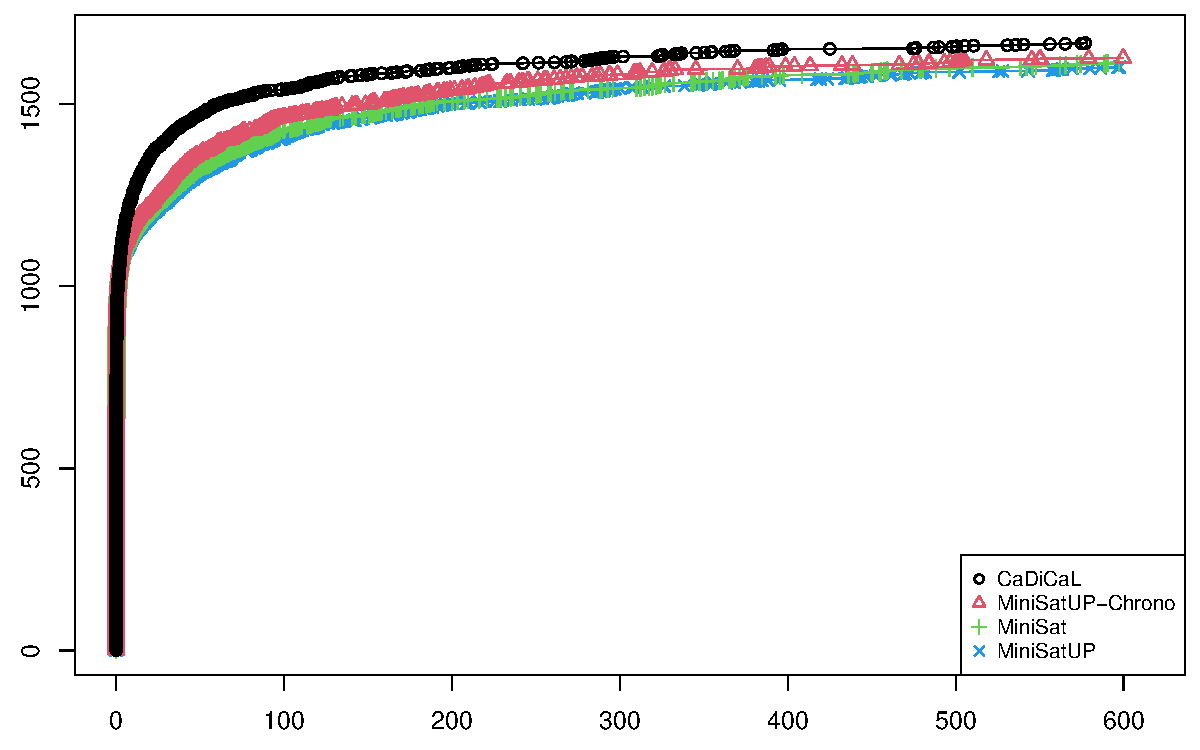
\includegraphics[width=0.85\linewidth]{plot.pdf}
    \caption{Accumulated solved instances (x-axis: running time in seconds, y-axis: number of solved instances)}
  \end{figure}
\end{frame}

\section{Summary and Future Work}
\begin{frame}{Summary}
  \begin{itemize}
    \item MiniSatUP: MiniSat extended with the IPASIR-UP interface
    \item Integrated MiniSatUP with cvc5
    \item Second implementation of IPASIR-UP after CaDiCaL
    \item Demonstrates practical, fine-grained SAT solver collaboration
    \item No performance overhead observed
  \end{itemize}
\end{frame}

\begin{frame}{Future Work}
  \begin{itemize}
    \item Investigate remaining failed and timeout cases in cvc5 integration
    \item Extend IPASIR-UP to support CaDiCaL-specific functions (termination, learned clause/fixed variable notification, resolution proof)
    \item Further abstract and simplify the SAT solver interface in cvc5 with IPASIR-UP
    \item Support proof validation in IDRUP format for MiniSatUP
    \item Further develop and optimize MiniSatUP with chronological backtracking
  \end{itemize}
\end{frame}

\begin{frame}[allowframebreaks]{References}
  \scriptsize
  \nocite{*}
  \bibliographystyle{abbrv}
  \bibliography{bibliography}
\end{frame}

\begin{frame}{Thank You}
  Questions?
\end{frame}

\end{document}
